\chapter{Design}
\label{chap:design}
This chapter describes the design of the whole platform in details, however, implementation specifics of some parts of the Distrace tool are described in the following Chapter \ref{chap:implementation}. The current chapter starts with the high-level overview of the complete platform and interactions between its parts. It is followed by a simple use-case to give the reader an idea how the Distrace tool is can be used.

Spans and their format are described next, followed by design of the native agent and instrumentation server. This chapter ends with description of the default Zipkin user interface and also JSON format, in which the user interface accepts the data from the instrumentation server. 

\section{Overview}
\label{design:overview}
The main purpose of the Distrace tool is to collect distributed traces. In order to achieve that, the Distrace tool is based on the concept of spans. Spans are used to denote some specific part of the communication between the communicating nodes and are important elements for building the whole trace trees. Trace trees consist of several spans and represent the complete task or communication, where a span inside the trace usually represents a few remote procedure calls between two neighboring nodes. The node initiating the trace creates so-called parent span and new calls started within the scope of this span create new nested spans. Created spans can be exported using different span exporters and can be sent to the user interface using various data collectors. Span exporters export spans in the desired format on disk or the network for further data collection. The collected data are used for spans visualization in the user interface. The user interface receives the spans from the span exporters or data collectors and presents them to the user in a form of trace trees.

Definition of when a new span is to be created and when an existing span needs to be closed is done by a developer by extending the core instrumentation server library. The created extended instrumentation server is then used for instrumenting the classes of the original application, however, spans are still located in the scope of the application itself. In order to obtain the class files for transformation, the native agent runs as part of the monitored application and sends the desired classes to the instrumentation server. The native agent is a core part of the whole platform. It is attached to the monitored application and additionally to providing the data to the instrumentation server, it is used to obtain various low-level information from the application. 

The Distrace tool, therefore, consists of three main components:
\begin{itemize}
	\item Native Agent
	\begin{itemize}
		\item Is used to obtain bytecode for the instrumentation.
		\item Is used to actually apply the instrumented bytecode.
	\end{itemize}
	\item Instrumentation Server
	\begin{itemize}
		\item Instruments the classes obtained from the native agent.
		\item Is also the base library for custom application instrumentation server.
		\item Can contain implementations of customized span exporters.
	\end{itemize}
	\item User Interface
\end{itemize}


The Figure \ref{fig:architecture} denotes the basic relationships between the major parts. Instrumentation server communicates with the native again, mainly in order to instrument classes. The application communicates with the user interface by sending the spans to it. The spans can be sent either via data collection agent or via one of the default span exporters explained later in this chapter. Each part is described in more detail later in this chapter. \begin{figure}
	\centering
	
\includegraphics[scale=0.6]{architecture.png}
	\caption{Basic relationship between the major components. }
	\label{fig:architecture}
\end{figure}

The Figure \ref{fig:full_overview} shows how trace trees and spans are related on a simple two nodes example. Each trace is separated from each other and represents tracing of a single computation, which consists of several spans. Spans denote more local computation and can also contain additional application-specific information. In order to connect the information from multiple nodes, the trace information needs to be attached to the node communication. That is also a reason why in this case the methods \texttt{send()}, \texttt{receive()} and \texttt{process()} need to be instrumented. These methods also open and close spans at the correct places in the code.
\begin{figure}
	\centering
	
\includegraphics[scale=0.56]{full_overview.png}
	\caption{Trace and span demonstration. }
	\label{fig:full_overview}
\end{figure}
\section{Example Use Case}
\label{design:use_case}
In order to demonstrate an use case for which this architecture may a good fit, a small example on a simple distributed application is shown in this section. The example consists of three modules. The client module used for submitting tasks, the execution module and the module used for exporting the data. These modules can be represented as separated threads in a single application or as different nodes of the distributed application. In this example, the user always passes a task to the client module. This module performs some pre-processing and sends the task to the execution module. This module performs the computation and once it's done, sends the data to the exporter module, which exports the data on disk and informs the client of the task completion. The architecture of the example can be seen on Figure \ref{fig:example_arch}.

The goal of this example is to record and visualize how long the transfers between different modules last and how long the processing on each module takes. It is also assumed that the platform does not collect this information already, otherwise the cluster monitoring tool would not be required. For simplicity, let's also assume that each module performs the functionality in a single method. The following code sections give the schematic code of each method.

	\begin{figure}
		\centering
		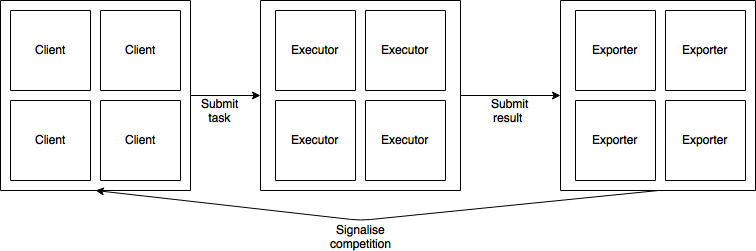
\includegraphics[scale=0.5]{example_arch.png}
		\caption{Example architecture.}
		\label{fig:example_arch}
	\end{figure}



\begin{itemize}
\item \textbf{The client:}
\begin{lstlisting}[language=Java]
public acceptTask(Task task){
  preprocessTask(task)
  ...
  sendTaskForComputation(task)
  ...
  waitForExporterToFinish()
  ...
}
\end{lstlisting}

\item \textbf{The executor:}
\begin{lstlisting}[language=Java]
public execute(Task task){
  TaskResult result = executeTask(task)
  ...
  sendResultForVisuzalization(result)
}
\end{lstlisting}

\item \textbf{The exporter:}
\begin{lstlisting}[language=Java]
public export(TaskResult result){
  saveToDatabase(result)
  ...
  notifyClient()
}
\end{lstlisting}
\end{itemize}

In order to collect this type of information and be able to reason about the relationship between the modules, these methods need to be instrumented. The instrumented code should look as in the schematic code below. Generally, the logic which keeps the track of the current trace and span needs to be injected into the code. To achieve this, developers are supposed to extend the core instrumentation server, which acts as the base library and provides them with several helper methods used to specify the instrumentation points for their applications. 

\begin{itemize}
\item \textbf{The instrumented client:}
\begin{lstlisting}[language=Java]
public acceptTask(Task task){
  TraceContext tc = TraceContext.create()
  tc.attachOnObject(task)
  Span s = tc.openSpan("Main Client Span")	
  s.addAnnotation("tskReceived", timestamp)
  ...
  preprocessTask(task)
  s.addAnnotation("tskPreprocessed", timestamp)
  ...
  sendTaskForComputation(task)
  ...
  Result res = waitForExporterToFinish() // blocking method
  ...
  tc.closeCurrentSpan()
}
\end{lstlisting}
The \texttt{create} method creates a new trace and the \texttt{attachOnObject} method attaches the trace context on the \texttt{task} object, which is passed around the network. The method \texttt{openSpan} opens a new span encapsulating the client computation. The \texttt{addAnnotation} method is used to add application specific information to the current span. The \texttt{closeCurrentSpan} method is used to close the current span and export the content using the provided span exporter. In the default case, the data are sent to the user interface directly.


\item \textbf{The instrumented executor:}
\begin{lstlisting}[language=Java]
public execute(Task task){
  TraceContext tc = TraceContext.getFromObject(task)
  tc.openSpan("Executor span")
  TaskResult result = executeTask(task)
  tc.attachOnObject(result)
  ...
  sendResultForExport(result) // non-blocking method
  tc.closeCurrentSpan()
}
\end{lstlisting}
In this case, we don't create a new trace context but obtain the existing one from the \texttt{task} object on the input. A new nested span is opened within the scope of the span, created in the previous module. The current span marks the span from the previous module as its parent.

\item \textbf{The instrumented exporter:}
\begin{lstlisting}[language=Java]
public export(TaskResult result){
  TraceContext tc = TraceContext.getFromObject(result)
  tc.openSpan("Exporter span")
  saveToDatabase(result)
  ...
  tc.closeCurrentSpan()
  notifyClient()	
}
\end{lstlisting}
In this case, the meaning of the methods is the same as above.

\end{itemize}

The developer should extend the base instrumentation server to instrument the classes in order to have a similar format as above. The extended instrumentation server is described on Figure \ref{fig:example_extended}.

	\begin{figure}
		\centering
		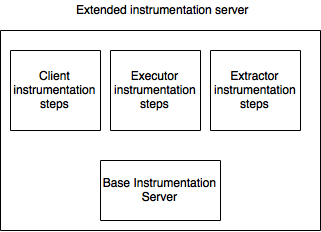
\includegraphics[scale=0.5]{example_extended.png}
		\caption{Structure of the extended instrumentation server JAR artifact.}
		\label{fig:example_extended}
	\end{figure}

The extended instrumentation server is run on each node or on the network and is used to perform the instrumentation requested from the application. The native agent has to be attached to all nodes of the distributed application prior its start and the path to the extended instrumentation server JAR needs to be set as the mandatory argument. The default span exporter is used in this case and the collected spans are sent right to the Zipkin user interface. The default IP address and port of the user interface are used when they are not explicitly configured as the native agent argument.

A single collected trace from this application should look as shown in Figure \ref{fig:example_trace}.

	\begin{figure}
		\centering
		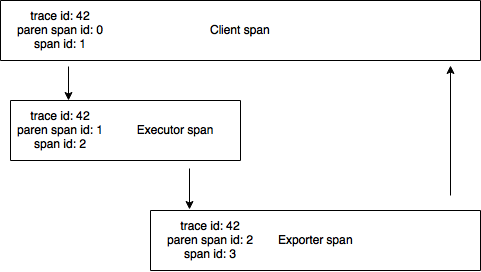
\includegraphics[scale=0.5]{example_trace.png}
		\caption{Example trace in case of the example application.}
		\label{fig:example_trace}
	\end{figure}

Therefore, it can be seen that the only part the developer needs to work on is the extension of the instrumentation server to specify the custom instrumentation points, otherwise the rest of technical work is done automatically. The end user is only responsible for starting the application with the agent attached.

\section{Spans and Trace Trees}
\label{subsec:spans}
As mentioned briefly in the previous section, spans are used to gather the information about the distributed calls or so called, distributed stack traces. Points in the code where spans are created and closed are defined as part of the instrumentation server but since it's the most important concept in the thesis, we explain them in the separated section. 

Spans are the main concept behind capturing the distributed traces. They are entities injected to the code of the instrumented application to keep track of the communication and state between the nodes of the distributed application. Usually, the initiator creates so called parent span and new calls started within the span create new nested spans. Collected spans can be processed using different span exporters and can be sent to the user interface using various data collectors.

Span has several mandatory and optional attributes. The mandatory attributes are trace id, span id and parent span id. Trace id identifies one complete distributed call among all interacting nodes of the cluster. This attribute is attached automatically when a new root span is created. A root span is the first span created inside the trace and does not have parent id attribute set up. Therefore, the user interface back-end can distinguish between regular spans and root spans and can identify the start of the whole trace. Parent id of a span is id of span in which scope the child span was created. The span and its parent span can be located on the same node or on different nodes as well. The first variant can be useful in cases where the developer requires to trace multiple threads as separated spans within a single application node.  

Span has also several additional optional fields, which are later used in the user interface. The fields are:
\begin{itemize}
	\item \textbf{Timestamp} - when the span started.
	\item \textbf{Duration} - how long the span lasted.
	\item \textbf{Annotations} - annotations used to carry additional timing information about spans. For example, time when the span has been received on the receiver side or the time the span has been processed at the receiver side can be set using these annotations.
	\item \textbf{Binary annotations} - annotations used to carry around application specific details. They can also be used to transfer information between communication nodes inside of a single span. For example, a sender can store number of bytes sent during the request and a receiver can use this information to calculate overall number of bytes received from this particular node.
\end{itemize}
Each span has also an internal field called \textbf{flags}. The developer may store tags important to the instrumentation and these flags are transferred as part of the spans. Flags are not sent to the user interface and are only used for instrumentation purposes. For example, they can be used in case of multiple spans exist at a single moment. In this case, these spans can be annotated with special flags and the decision can be made based on this to process these spans.

Each annotation, both binary and regular, has also an endpoint information attached. This element consist of:
\begin{itemize}
	\item \textbf{IP} - IP of the node on which this event was recorded.
	\item \textbf{port} - port of the service which recorded the span.
	\item \textbf{service name} - a special name, which is used in the user interface to group and filter different traces by names.
\end{itemize}

\subsection{Span IDs}
It is also important to mention that span id is created randomly. This is done in order to allow parallel spans to coexist in the same control flow without overlapping as can be seen on Figure \ref{fig:parallel_spans}.

	\begin{figure}
		\centering
		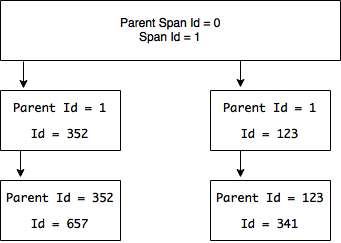
\includegraphics[scale=0.6]{parallel_spans.png}
		\caption{Generating span ids randomly ensures that they don't overlap when they are created in parallel.}
		\label{fig:parallel_spans}
	\end{figure}
If the ids were not random at different nodes of the distributed system, the parallel spans would be creating child spans with ids in the same linear sequence and therefore these spans would be overlapping, as can be seen on Figure \ref{fig:parallel_spans_overlapping}
	\begin{figure}
		\centering
		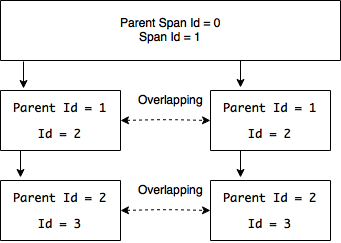
\includegraphics[scale=0.6]{parallel_spans_overlapping.png}
		\caption{Generating span with the same linear sequence leads to span overlapping.}
		\label{fig:parallel_spans_overlapping}
	\end{figure}
	
The following sections contain information about how spans are exported for processing outside of the Distrace tool and also how spans are created using \texttt{TraceContext} and \texttt{TraceContextManager}.
\subsection{Span Exporters \& Data Collectors}
\label{design:exporter}
Spans can be exported from the application using so called span exporters. The type of the exporter can be configured via one of the native agent configuration properties. It is important to mention that the exporter is configured globally and each span in the application is using the same exporter\footnote{Exporter is a static attributed of the \texttt{Span} entity.}. The monitored application needs to have the chosen span exporter available at run-time, since the export is performed at the scope of the monitored application. Therefore, exporters are sent to the native agent during the initialization phase and the agent puts the exporters on the application classpath.

The Distrace tool includes two default implementation of span exporters, but also allows the developer to create new span exporters. Custom span exporters may be useful in cases when the developer wants to export the span data in a format used by different user interface or to use custom data collector. Data collector is a service, which collects data from the specified location and stores them in a central data storage available to all nodes in the distributed application. The Distrace tool does not implement data collection service as many services exist for this purpose. 

Data collected within spans are internally represented in JSON format understandable to the Zipkin user interface. This is also the reason why Distrace contains support for working with JSON data and it is explained in more detail later in Section \ref{json_gen}. This output format can be customized by the custom span exporter.

The implementation details are available at Section \ref{imp:exporter}.
\subsection{Trace Context}
Trace context is used for storing the information about the current span and also for creating new spans and closing current spans. Trace context can be attached to a specific object and thread. This is done in order to allow multiple threads to have different computation state and therefore the platform is able to capture multiple distributed traces at the same time on the same node. Trace context manager is used for attaching trace context to threads and vice-versa. It provides several operations allowing to the developer to attach trace context to a specific thread and also to get trace context from a specific thread.

Each trace is represented by trace context and is uniquely identified by Universally unique identifier (UUID) of type one\footnote{More UUID versions exist and are created based on different information}. This UUID type combines 48-bit MAC address of the current device with the actual timestamp. This way it is ensured that two traces created at the same time on different nodes can not have the same identifier. The identifiers are generated in the native agent using C++ library called Sole\footnote{The Sole library is available at \url{https://github.com/r-lyeh/sole} and can be used to create identifiers in C++ language.} and are made available to the Java code via published native operation \texttt{getTypeOneUUID}.

The trace contact has \texttt{openNestedSpan} and \texttt{closeCurrentSpan} operations. The first operation is used to create a new nested span and set the newly created span as the current one. Nested span is opened within the scope of its parent span and remembers the parent span. A root span is created in case no current span exists. The second operation is used to close the current span.

The second operation closes the the current span. This consist of two actions. The current span is exported using the configured span exporter and the parent span becomes the current span. The Figure \ref{fig:closing_spans} shows how spans are created, closed and exported. \begin{figure}
	\centering
	
\includegraphics[scale=0.6]{closing_spans.png}
	\caption{Creating and closing spans.}
	\label{fig:closing_spans}
\end{figure}

\subsection{Transferring Span Information}
In order to capture the shared state between the nodes in the distributed application or between the threads on the same application node, the span details and trace context have to be transferred between the threads or the nodes. Distrace prepares several operations for attaching trace context to either a current thread or to an object acting as the carrier of the trace information.

Usually when transferring the trace context between the threads on the same node, the copies of the trace context should be used. This is not an issue when transferring the trace context between the different nodes of the distributed application.


The developer responsible for extending the instrumentation server can use operations like:
\begin{itemize}
	\item  \texttt{getTraceFromThread}
	\item \texttt{getTraceFromObject}
	\item \texttt{attachTraceToThread}
	\item \texttt{attachTraceToObject}
\end{itemize}
More information about the trace context API is available at \ref{imp:trace_context_api}.

There are also different variants of how spans can be closed. A span can be closed by the same node or thread who created it. In this case, attaching the trace context information to the current thread is usually sufficient. However, it is also possible that the span can be closed by different thread or node that originally created this span. In this case, the copy of the trace context should usually be created and attached to the object, which is used as the carrier of the trace context.
\section{Native Agent}
\label{native_agent_design}
The native agent is used for accessing the internal state of the monitored application and also to instrument classes so they can carry the span and trace identifiers between the application nodes. The main task of the agent is to check whether a class is required to be instrumented and if yes, send the class for the instrumentation to the server and wait for the instrumented code.

The native agent consist of several modules. The most important ones are:
\begin{itemize}
	\item \textbf{Bytecode parsing module}. \newline The classes in this module are used to parse the JVM bytecode in order to discover the classes dependencies for further instrumentation. Byte code parsing is a technical task described in Section \ref{imp:parsing}.
	\item \textbf{InstrumentorAPI}. \newline The \texttt{InstrumentorAPI} class provides several methods, which are used to communicate with the instrumentation server JVM. All the queries to the server go through the instance of this class.
	\item \textbf{AgentCallbacks}. \newline All callbacks used in the native agent are defined in this namespace.
	\item \textbf{AgentArgs}.  \newline The \texttt{AgentArgs} class contains all the logic required for argument parsing.
	\item \textbf{NativeMethodsHelper}. \newline The \texttt{NativeMethodsHelper} class is used for registering native methods defined in C++. These methods can be used from the Java code without worrying about the low-level implementation.
	\item \textbf{Utilities module}. \newline This module contains several utility namespaces. The most important are \texttt{AgentUtils} and \texttt{JavaUtils} namespaces. The first contains methods for managing the JVMTI connection and for registering the JVMTI callbacks and events. The second is used to simplify work with Java objects in the native code via JNI.
\end{itemize}

\subsection{Agent Initialization}
\label{desing:native_initialization}
The agent is initialized through the same phases as described in Section \ref{subsec:jvmti_init}. The following JVMTI events are especially important to the thesis: \texttt{VM Init}, \texttt{VM Start}, \texttt{VM Death}, \texttt{Class File load Hook}, \texttt{Class Prepare} and \texttt{Class Load}. Callbacks are registered for all the mentioned events so the native agent can react to them accordingly in the code.

As part of the initialization process, the agent is responsible for either connecting to or starting a new instrumentation server. In case the native agent was started in the shared mode of the instrumentation server, the agent tries to connect to already existing server and the server is shared between all  nodes of the distributed application. In the local instrumentation mode, the server is started as a separated process automatically and the connection is established with the server using the inter process communication. In this case, each application node has dedicated instrumentation server.

The callback registered for the \texttt{VM Init} event is responsible for loading all additional classes from the instrumentation server as part of the initialization as well. The additional classes are for example \texttt{Span}, \texttt{TraceContext} or custom implementations of \texttt{SpanExporter} abstract class. These classes need to be available at run-time at the monitored application. They are required since the instrumented code is using trace context and spans for preserving the information about the current trace and the exporters for exporting the spans from the application. Therefore, these classes have to be available at the monitored application. The native agent is designed in a way that developers are not supposed to change the code of if. All the extension are supposed to be done as part of the extended instrumentation server. Therefore, the server is asked at the initialization phase for the list of all additional classes and they are sent to the native agent. The agent puts all the received classes on the application's classpath so they are available to the instrumented code.

\subsection{Instrumentation}
Code for handling the instrumentation is part of the callback for the \texttt{Class File load Hook} event. The callback has the bytecode for the class being loaded as its input parameter and allows the developer to pass a new instrumented bytecode as the output parameter. The process of instrumentation is described at this section, however some technical details are described in Chapter \ref{chap:implementation}.

The process consist of several stages:
\begin{enumerate}
	\item Enter \texttt{Class File load Hook} callback.
	\item Enter the critical section. It can happen that the class file load hook is triggered multiple times and to prevent confusing the instrumentation server, the lock has to be acquired before the instrumentation of a class starts.
	\item Firstly, we check whether the virtual machine with the application is \linebreak started. If the JVM is initialized, the instrumentation continues, otherwise the instrumentation for currently a class currently being loaded is skipped. In this case, the instrumentation server is not contacted since the classes being loaded are at this point system classed and it is not desired to instrument Java system classes.
	\item Attach JNI environment to the current thread. Since the JVMTI and JNI does not have automatic thread management, it is up to the developer to take care of correct threading management.
	\item Discover the class loader which is loading the class.
	\item Parse name of the class currently being loaded and the nape of the class loader loading the current class. Even though the callback provides input parameter, which should contain the name of the class, at some circumstances it can be set to \texttt{NULL} even though the class name is available in the bytecode. Instead of relying on this parameter, the bytecode is parsed and the class name is found manually.
	\item Decide whether the instrumentation should continue. This check is based on the used class loader and name of the class being loaded. Classes loaded by the \texttt{Bootstrap} class loader and in case of Oracle JVM, classes loaded by \texttt{sun.reflect.DelegatingClassloader} are not supposed to be instrumented. 
	The \texttt{Bootstrap} class loader is used to load system classes and the second mentioned class loader is used to load synthetic classes. and in both cases, it's not desired to instrument classes loaded by these class loaders.
	There are also some ignored classes for which the instrumentation is not desired. For example, classes loaded during initialization phase from the instrumentation server and the auxiliary classes generated by the Byte Buddy framework should not be instrumented. Auxiliary classes are small helper classes Byte Buddy is using for example to access the super class of the currently being instrumented class. Therefore, the instrumentation continues only if the class is not ignored and not loaded by any of the ignored class loaders.
	
	\item The instrumentation server is asked whether the class is marked for instrumentation. The agent does not know which classes are to be instrumented and therefore, it needs to query the server. The classes to be instrumented are marked by developer when extending the instrumentation server library using simple Byte Buddy API. The process ends if the class should not be instrumented.
	
	\item Check whether the instrumentation server already contains the class being loaded. If the server contains the class, we go to the next step and wait for the instrumented class. If the server does not contain the class, the native agent sends the class data to the instrumentation server, parse the class file for all the dependent classes and send all dependent classes for the instrumentation. This step is repeated through all dependencies recurrently until the loaded class does not have any other dependencies or until all dependencies are already available on the server. All dependencies for the currently instrumented class have to be available on the server in order to perform the instrumentation.

	\item At this stage, the class is already on the instrumentation server and all dependencies for this class as well. The native agent waits for the instrumented bytecode to be sent from the server and sets the modified bytecode as the output argument of the \texttt{Class File load Hook} callback.
	
	\item Exit the critical section.
	\item Exit \texttt{Class File load Hook} callback.
\end{enumerate}
The Figure \ref{fig:inst_state} is the state machine diagram representing the instrumentation steps, where the numbers in selected steps correspond to the items in the list above.
	\begin{figure}
		\centering
		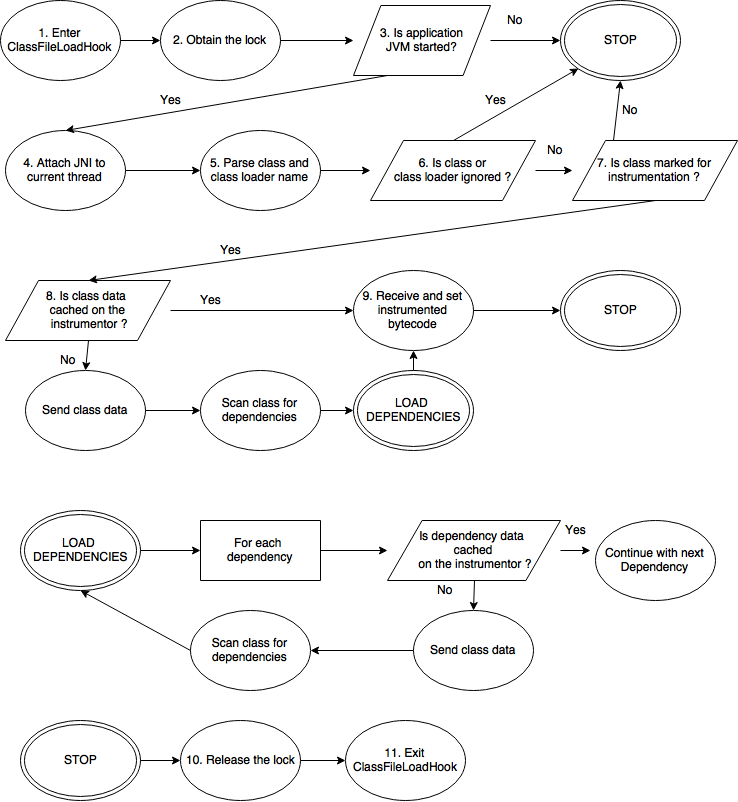
\includegraphics[scale=0.55]{inst_state.png}
		\caption{State machine diagram representing the instrumentation process.}
		\label{fig:inst_state}
	\end{figure}
	
Several technical difficulties had to be dealt with during the development. For example, cyclic dependencies between classes need to be properly handled during the instrumentation. We need to also ensure that the dependencies for instrumented classed are also instrumented in the correct order. The final solution to these problems is described in Section \ref{imp:native:inst}

The behavior of the agent may be configured using the arguments passed to the agent. Please see the Attachment 4 for the full list of native agent arguments.

\section{Instrumentation Server}
\label{sec:inst_server}
The instrumentation server is responsible for instrumenting the bytecode received from the native agent in separated JVM and it also acts as the base library for instrumenting specific applications. The developer extending the instrumentation server can use prepared operations to define custom instrumentation points without touching the internals of the native agent.

This section covers several design aspects of the instrumentation server, leaving the implementation details on the following sections. The core instrumentation on the server is handled by the Byte Buddy code manipulation framework. The native agent asks the server if the class currently being loaded is required to be instrumented. If yes, the server receives the bytecode, performs the instrumentation and sends the data back to the agent. The server does not contain any application state, in particular it does not take track about the distributed traces. The information about traces is contained in the instrumented classes within the monitored application.

The platform was designed to be configurable and deployment of the instrumentation server is supported via two approaches. The instrumentation server can be located either on the network to all nodes of the distributed application and can be shared by all nodes. This has the advantage of caching the instrumented classes. When any class is instrumented for the first time based on request from any node, it is saved and the instrumentation is not performed for other nodes. Instead, the class can be sent immediately. The disadvantage of this solution is higher latency between the agent and the instrumentation server since they are usually not on the same physical node. In this case, the instrumentation server has to be manually started in advance. Architecture of this scenario is depicted on Figure \ref{fig:shared_server}.
 
 \begin{figure}
 	\centering
 	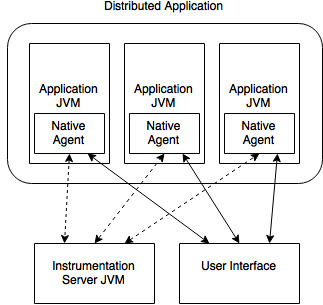
\includegraphics[scale=0.8]{shared_server.png}
 	\caption{Architecture with the shared instrumentation server. The dotted lines represent the communication between the server and the agent, whilst the regular lines represent data transfer from the agent to the user interface.}
 	\label{fig:shared_server}
 \end{figure}
 
 The other deployment method is that the instrumentation server runs on each node of the distributed application. This has the advantage of faster communication since in this case, inter-process communication is used to communicate between monitored JVM and the instrumentation server. The disadvantage of this solution is that all classes have to be instrumented on each node since there is no communication between the instrumentation servers. In this solution, the server is started automatically during the native agent initialization. Architecture of this scenario is depicted on Figure \ref{fig:separated_server}.
 
 \begin{figure}
 	\centering
 	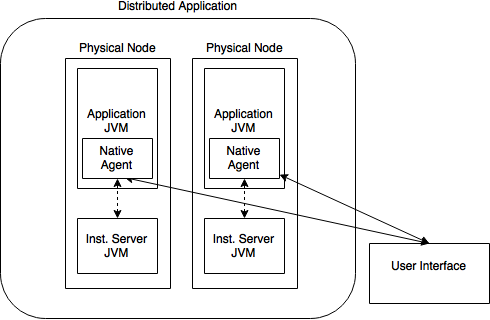
\includegraphics[scale=0.8]{separated_server.png}
 	\caption{Architecture with separated instrumentation server. The dotted lines represent the communication between the server and the agent, whilst the regular lines represent data transfer from the agent to the user interface.}
 	\label{fig:separated_server}
 \end{figure}

Except from the cached classes, the server does not contain any application state and it just reacts to the agent requests. It can accept four type of requests:
\begin{itemize}
	\item Request for code instrumentation.
	\item Request to store bytecode for a class on the server.
	\item Request to send all helper classes needed by the agent such as the \texttt{Span} class or \texttt{TraceContext} class.
	\item Request to check whether the server contains specific class or not.
\end{itemize}
The server interacts in more ways with the agent, however all communication is initiated by one of these four request types.	

The instrumentation server needs to deal with several technical problems. The main issue is that the classes, which are about to be instrumented, require all other dependent classes to be available. The other issue is instrumenting the classes with circular dependencies. The server also performs several optimizations to provide faster response to the agent such as caching the instrumented classes and minimizing the communication when possible. The technical aspects of these issues and the optimizations mentioned above are described in Chapter \ref{chap:implementation}.
\subsection{Instrumentation}
The instrumentation of the class is triggered by the agent and it's done in two stages. The first stage informs the agent whether the class is already available on the instrumentation server or not. The second stage is the instrumentation step itself. The first stage is initiated by the agent and the server performs the check for class availability in three phases:
\begin{enumerate}
	\item Check if the instrumented bytecode for this class is available.
	\item If not, check if the original bytecode for this class is available.
	\item If not, check if the class can be loaded using the server's context class loader. This handles the cases where the user builds the instrumentation server together with the application classes or adds the classes on the server classpath for optimization reasons.
\end{enumerate}

The server informs the agent if it does not have the bytecode for the class available. In that case, the agent sends the class to the server and the server registers the received bytecode under the class name. Therefore, the agent does not have to send the class next time since it's already cached on the instrumentation server.
The second stage follows the first stage immediately. If the server already contains the instrumented class in the cache, the transformed class is sent right away without instrumenting the class again. If the cache is empty, the class is instrumented and put into the cache.

More information about instrumentation process on the server is described in more details in Section \ref{impl:server:instr}.
\subsection{Custom Service Loader}
Service loaders are used for loading the extensions to the Distrace tool and creating the extended instrumentation server. The service loader is used for two object types: 
\begin{itemize}
	\item \textbf{Custom span exporters} - Each span exporter inherits from the abstract \texttt{SpanExporter} class.
	\item \textbf{Custom Interceptors} - Each interceptor has to implement the interface \texttt{Interceptor}.
\end{itemize} 
The user can create custom span exporters and interceptors by either inheriting the desired class or implementing the required interface. In order to allow the platform to locate the custom implementations, the name of the class has to be written inside the text file in the META-INF directory in the extended instrumentation server JAR file. The text file has to have the same name as the abstract class or the interface the particular implementation is for. For example, when the user creates a new interceptor called \texttt{x.y.InterceptorA}, the file \texttt{Interceptor} in the META-INF folder has to contain line \texttt{x.y.InterceptorA}.

Java provides service loader for this purpose. However the standard Java implementation looks up the classes defined as above and automatically creates new instances using the well-known constructors. For the thesis purposes this was unwanted as it is only required to obtain \texttt{Class} object representing the available implementation. Therefore a custom service loader was created. This service loader works in very similar way as the standard Java implementation, but instead of returning the instances of loaded services, it just returns classes representing the available services. 

\section{User Interface}
\label{sec:zipkin_ui}
The user interface receives spans and presents them in a hierarchical way so the relationships between different nodes can be seen easily. The important feature of the user interface is that the data for a single span can be sent incrementally. This means that several JSONs representing the same span can be sent with different annotations and the user interface merges these spans into single one and presents all annotations under the given span. This allows the Distrace tool to send part of data from the sender side and part of data from the receiver side directly to the user interface, instead of sending the data back and forth to send them as one single complete span.

The Distrace tool is using Zipkin as default user interface. The default format for exporting spans is designed in order to be understandable by this user interface. The user is however still able to change the data format to support custom user interface via custom span exporters. This section gives an overview of Zipkin user interface and describes the Zipkin data model. The example output of a single trace in the Zipkin user interface can be seen on Figure \ref{fig:zipkin_ui}.

\begin{figure}
	\centering
	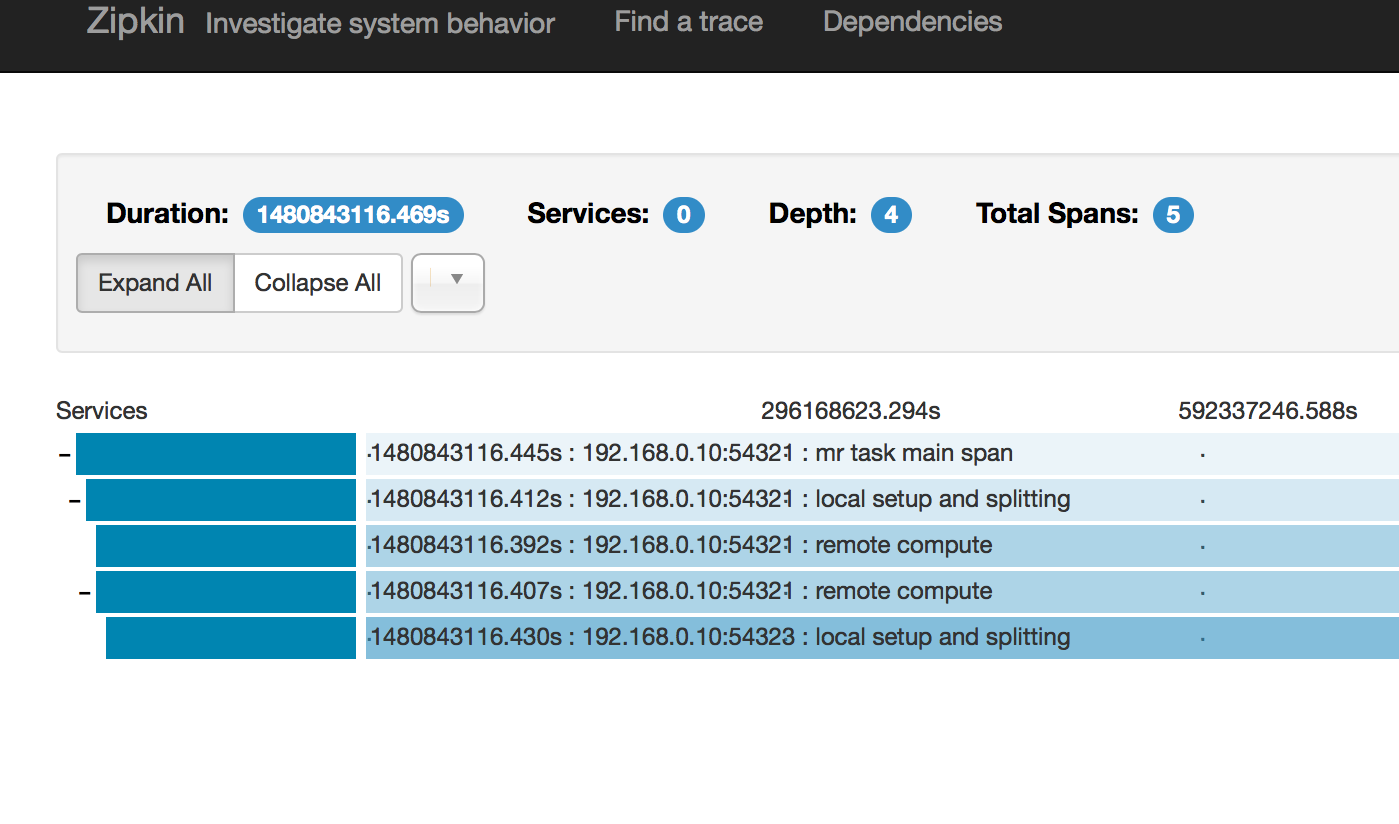
\includegraphics[scale=0.5]{zipkin_ui_example.png}
	\caption{Example of trace output in the Zipkin user interface.}
	\label{fig:zipkin_ui}
\end{figure}

Each span in the user interface is clickable and all the additional information can bee seen at that level. The Distrace tool also automatically collects the stack trace at the time of span creation and closing. Example of such information screen can be seen on Figure \ref{fig:zipkin_ui_detail}.
\begin{figure}
	\centering
	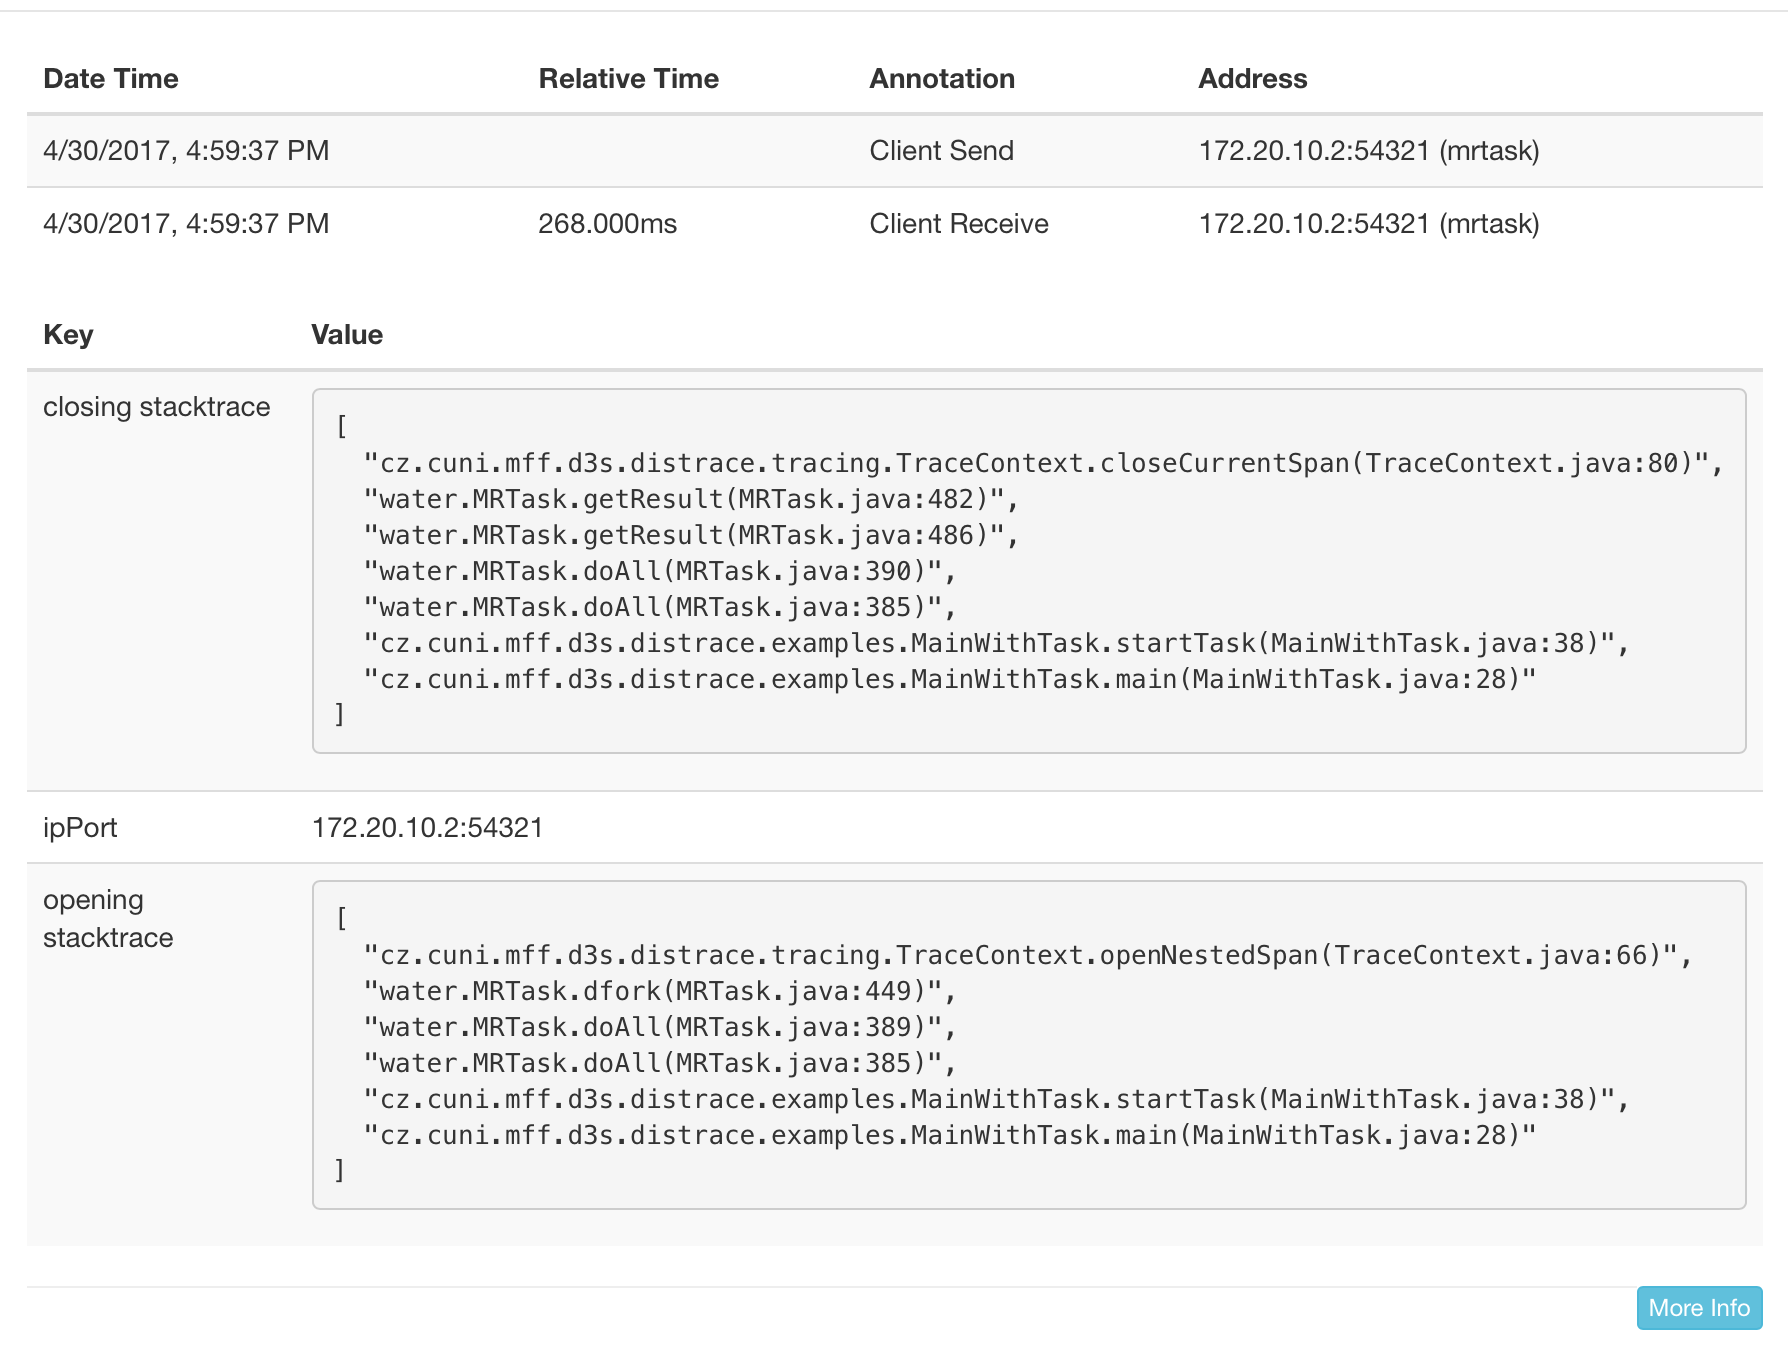
\includegraphics[scale=0.4]{zipkin_ui_detail.png}
	\caption{Example of the detail span information.}
	\label{fig:zipkin_ui_detail}
\end{figure}
\subsection{Zipkin Data Model}
Zipkin requires data to be sent in JSON format. Requests to the user interface are sent as JSON arrays, where the array elements are the spans. Zipkin understands the following attributes of span object:
\begin{itemize}
	\item \textbf{traceId} - unique id representing the complete trace. It can be either 128 or 64 bit long.
	\item \textbf{name} - human readable span name.
	\item \textbf{id} - id of this span. At the current implementation, Zipkin user interface supports span ids only to be 64-bit long.
	\item \textbf{parentId} - parent id of the current span.
	\item \textbf{timestamp} - the time of the span creation.
	\item \textbf{duration} - the duration of the span. It is the duration between the span creation and closing.
	\item \textbf{annotations} - array containing standard Zipkin annotations. These annotations can be handled by the user interface in a specific way, since the user interface understands the meaning of content of these annotations. Following annotations are available:
	\begin{itemize}
		\item \textbf{cr} : timestamp of client receiving the span.
		\item \textbf{cs} : timestamp of client sending the span.
		\item \textbf{sr} : timestamp of server receiving the span.
		\item \textbf{ss} : timestamp of server sending the span.
		\item \textbf{ca} : client address.
		\item \textbf{sa} : server address.
	\end{itemize}
	\item \textbf{binaryAnnotations} - array of custom annotations. For example, collected stack traces are sent as a binary annotation.
\end{itemize}

Except the \textbf{annotations} and \textbf{binaryAnnotations} attributes, the attributes are of simple string or number type. Annotations are objects consisting of three additional attributes - annotation value, annotation name and the endpoint. Endpoint is another object specifying the address and port of the node in the distributed application, where the span or particular annotation was recorded. Endpoints can also specify service name, which may be used to search for particular spans. Full example of data sent to Zipkin user interface can be:
\begin{lstlisting}[emph={traceId, name, id, timestamp, duration, annotations, value, endpoint, serviceName, ipv4, port, binnaryAnnotations, key},emphstyle={\textbf}]
[
 {
    "traceId": "123456789abcdef",
    "name": "query",
    "id": "abcd1",
    "timestamp": 1458702548467000,
    "duration": 100743,
    "annotations": [
      {
        "timestamp": 1458702548467000,
        "value": "sr"
        "endpoint": {
          "serviceName": "example",
          "ipv4": "192.168.1.2",
          "port": 9411
        },
      }
    ],
    "binaryAnnotations": [
      {
        "key": "bytes_sent",
        "value": "1783"
        "endpoint": {
          "serviceName": "example",
          "ipv4": "192.168.1.2",
          "port": 9411
        },
      }
    ]
 }
]
\end{lstlisting}


